%!TEX TS-program = lualatex
%!TEX encoding = UTF-8 Unicode

\documentclass[12pt]{exam}
\usepackage{graphicx}
	\graphicspath{{/Users/goby/Pictures/teach/163/lab/}} % set of paths to search for images

\usepackage{geometry}
\geometry{letterpaper, bottom=1in}                   

\usepackage{afterpage}
\usepackage{pdflscape}

\newlength{\myindent}
\setlength{\myindent}{\parindent}
\newcommand{\ind}{\hspace*{\myindent}}


%\geometry{landscape}                % Activate for for rotated page geometry
\newlength{\litindent}
\setlength{\litindent}{\parindent}

\usepackage[parfill]{parskip}    % Activate to begin paragraphs with an empty line rather than an indent
%\usepackage{amssymb, amsmath}
%\usepackage{mathtools}
%	\everymath{\displaystyle}

\usepackage{fontspec}
\setmainfont[Ligatures={TeX}, BoldFont={* Bold}, ItalicFont={* Italic}, BoldItalicFont={* BoldItalic}, Numbers={OldStyle,Proportional}]{Linux Libertine O}
\setsansfont[Scale=MatchLowercase,Ligatures=TeX, Numbers=OldStyle]{Linux Biolinum O}
\setmonofont[Scale=MatchLowercase]{Inconsolatazi4}
\usepackage{microtype}

\usepackage{unicode-math}
\setmathfont[Scale=MatchLowercase]{Asana Math}
%\setmathfont[Scale=MatchLowercase]{XITS Math}

% To define fonts for particular uses within a document. For example, 
% This sets the Libertine font to use tabular number format for tables.
\newfontfamily{\tablenumbers}[Numbers={Monospaced}]{Linux Libertine O}
\newfontfamily{\libertinedisplay}{Linux Libertine Display O}

\usepackage{longtable}

\usepackage{booktabs}
\usepackage{multirow}
\usepackage{multicol}

\usepackage[justification=raggedright, labelsep=period]{caption}
\captionsetup{singlelinecheck=off}
\captionsetup{skip=0.2em}

%\usepackage{tabularx}
%\usepackage{siunitx}
\usepackage{array}
\newcolumntype{L}[1]{>{\raggedright\let\newline\\\arraybackslash\hspace{0pt}}p{#1}}
\newcolumntype{C}[1]{>{\centering\let\newline\\\arraybackslash\hspace{0pt}}p{#1}}
\newcolumntype{R}[1]{>{\raggedleft\let\newline\\\arraybackslash\hspace{0pt}}p{#1}}

\newcolumntype{M}[1]{>{\centering\let\newline\\\arraybackslash\hspace{0pt}}m{#1}}

\usepackage{tikz}

\usepackage{enumitem}
\setlist{leftmargin=*}
\setlist[1]{labelindent=\parindent}
\setlist[enumerate]{label=\textsc{\alph*}., ref=\textsc{\alph*}}

%\usepackage{hyperref}
\usepackage{hanging}

\usepackage[sc]{titlesec}


\renewcommand{\solutiontitle}{\noindent}
\unframedsolutions
\SolutionEmphasis{\bfseries}

\renewcommand{\questionshook}{%
	\setlength{\leftmargin}{-\leftskip}%
}
%Change \half command from 1/2 to .5
%\renewcommand*\half{.5}


\makeatletter
\def\SetTotalwidth{\advance\linewidth by \@totalleftmargin
\@totalleftmargin=0pt}
\makeatother



\pagestyle{headandfoot}
\firstpageheader{BI 063: Evolution and Ecology}{}{\ifprintanswers\textbf{KEY}\else Name: \enspace \makebox[2.5in]{\hrulefill}\fi}
\runningheader{}{}{\footnotesize{pg. \thepage}}
\footer{}{}{}
\runningheadrule

\newcommand*\AnswerBox[2]{%
    \parbox[t][#1]{0.92\textwidth}{%
    \begin{solution}#2\end{solution}}
    \vspace{\stretch{1}}
}

\newenvironment{AnswerPage}[1]
    {\begin{minipage}[t][#1]{0.92\textwidth}%
    \begin{solution}}
    {\end{solution}\end{minipage}
    \vspace{\stretch{1}}}

\newlength{\basespace}
\setlength{\basespace}{5\baselineskip}

\newcommand{\allele}[1]{\textit{#1}}

%\printanswers

\begin{document}

\subsection*{Natural selection in bacteria}

All species can evolve through the process of natural selection, including bacteria. Modern bacteria are frequently exposed to chemical agents, such as antibiotic drugs and antimicrobial soaps, as humans attempt to control bacterial disease and contamination. Many bacteria have evolved resistance to common agents intended to control bacteria. For example, about 94\% of the different strains of \textit{Staphylococcus aureus}, a common source of staph infections, were killed by penicillin when the drug was introduced in the early 1940s. In less than a decade, only 50\% of strains were susceptible. Within another decade, severe outbreaks of \textit{S. aureus} in hospitals were common (Livermore 2000). \textit{Staphylococcus aureus} and other bacteria evolved resistance to penicillin through natural selection. As bacteria were exposed to penicillin, many individuals were killed but not all. Surviving individuals were still able to reproduce so they had higher relative fitness. As the survivors reproduced, their offspring inherited resistance to penicillin. 

Imagine you are infected by just one cell of a harmful bacterium. Bacteria are capable of dividing (reproducing) every 20 minutes. Each division produces two cells from one parent cell. In 10 hours, the total number of bacteria from 30 divisions would be $2^{30} = 1,073,741,824,$ more than one billion cells. (No wonder illness seems to set in so quickly.) Now that you are feeling poorly, you take an antibiotic labeled as 99.9\% effective. The antibiotic might kill most cells but as many as 1,073,741 cells (0.01\% of 1,073,741,824 cells) might not killed by the antibiotic. \emph{Each} of those one million cells could go on to produce another one billion cells within 24 hours (the antibiotic can slow the growth of resistant bacteria), each with some resistance to the antibiotic. The problem is magnified because some people take antibiotics only until they feel better instead of the full time prescribed. An incomplete dose allows even more resistant bacterial cells to survive that might have been killed if the full dose had been taken. 

For this lab, you will expose a harmless soil bacterium, \textit{Bacillus cereus,} to different concentrations of Triclosan, an antimicrobial drug that was once used in hand soaps at concentrations of 0.1–0.4\%. You will test the ability of four concentrations of Triclosan (0.1\%, 0.3\%, 0.5\%, and 0.7\%) to inhibit growth of \textit{B. cereus.} You will grow the bacterium on agar plates. You will place a paper disk soaked with Triclosan in the center of the agar plate. The drug will seep into the agar, potentially inhibiting the growth of the bacteria around the disk. The inhibiting effect will decrease farther away from the disk so some bacteria will be able to survive if they are far enough away. You will measure the diameter of the zone of inhibition to determine the inhibitory effect of the drug. The Triclosan is dissolved in 50\% ethanol so you will include a control of 50\% ethanol without the drug.

\begin{questions}

\question
Write a hypothesis. How do you think different concentrations will affect the growth of \textit{B. cereus?}

%\vspace*{3\baselineskip}
\newpage

\question
Turn your hypothesis is a prediction. Remember that your prediction should predict the results of the experiment that would support your hypothesis. 

\vspace*{3\baselineskip}

\subsubsection*{Materials}

Everyone at your table will work as one group. Each table has the following items. Check to be sure each item is present before you begin. If you are missing an item, notify your instructor immediately.

\begin{itemize}

	\item Five petri plates with LB agar.
	
	\item One test tube culture of \textit{Bacillus cereus.}
	
	\item Four small jars of Triclosan at concentrations of 0.1\%, 0.3\%, 0.5\% and 0.7\%, dissolved in 50\% ethanol.
	
	\item One small jar with 50\% ethanol. This is a control.

	\item Glass petri dish of paper disks.
	
	\item Forceps.
	
	\item One biohazard bag.
	
	\item Sterile swabs.
	
	\item Non-latex gloves.
	
	\item A marker for labeling.
	
\end{itemize}

\subsubsection*{Procedure}

	\begin{enumerate}
	
		\item Decide on a catchy but easy to remember name for your group. 
	
		\item Label the \emph{bottoms} of five petri plates with your catchy group name and your lab section number. \emph{Write the information near one edge so it will not obstruct your ability to take measurements next week.} Your instructor will tell you your section number.
		
		\item Label the \emph{top} of each petri plate with either C, 0.1\%, 0.3\%, 0.5\%, or 0.7\%, for the control and each of the four Triclosan concentrations. 
		
		\item Put on a pair of gloves. \label{swab_first} Remove one sterile swab from the wrapper. 
		
		\item Remove the cap from the test tube culture of \textit{B. cereus.} Dip the cotton tip into liquid and remove. Place the cap back on the tube. Do \emph{not} dip the swab back into the culture.
		
		\item Carefully lift the lid off the petri plate enough to reach the entire surface of the agar with the swab.
		
		\item Swab the surface of the entire surface of the agar. Use gentle sweeping strokes to cover the entire surface. Rotate the plate 90° and swab again to cover the entire surface with bacteria. Do \emph{not} dip the swab back into the culture.
		
		{\centering\includegraphics[height=1in]{petri_plate_swab}\par
		}
		
		\item \label{swab_last} Close the lid and place the swab into the provided biohazard bag.
		
		\item Repeat steps~\ref{swab_first}–\ref{swab_last} for the other four petri plates. \emph{Use one new swab per plate.}
		
		\item \label{disk_first} Use sterile forceps to carefully remove one sterile disk from the glass petri dish. Dip the disk into the the microcentrifuge tube labeled C for one second and remove. This is control solution.
		
		\item \label{disk_last} Carefully lift the lid from the petri dish labeled C. Carefully lay the wet disk in the center of the petri plate. Place the lid back on the plate.

%		{\centering\includegraphics[height=1in]{petri_plate_disks}\par
%		}

		\item Repeat steps~\ref{disk_first}–\ref{disk_last} for each of the four concentrations of Triclosan.
		
		\item Place your petri plates in a stack \emph{upside down} on the counter at the back of the room.
		
	\end{enumerate}

The bacteria will be allowed to grow at room temperature for 24–48 hours. Your instructor will move the plates to a refrigerator to inhibit continued bacterial growth until you collect your data in lab next week.

\subsubsection*{Data collection}

\begin{enumerate}

	\item Find your petri plates on the back counter and bring them to your table.
	
	\item Each plate should have, starting from the center, a clear zone of inhibition around the disk where no bacterial colonies are growing, a “halo” with scattered bacterial colonies growing, and then a solid bacterial “lawn,” as shown in the figure below.
	
		{\centering\includegraphics[height=1.25in]{petri_plate_results}\par
		}

	\item Place the plates on your table with the top side down to take measurements. \emph{Do not open the plates to take measurements.}
	
	\item Measure the diameter in centimeters of the zone of inhibition with the ruler (horizontal line in the figure below). You will have to estimate the boundary between the zone of inhibition and the halo. Record the measurement in the table below. Measure the diameter of the halo (vertical line). Record the measurement in the table. You do have to hold the ruler at the same angles as indicated in the figure. Do this for all five plates.

		{\centering\includegraphics[height=1.25in]{petri_plate_measure}\par
		}

	\item After you have your measurements, return your plates in a stack to the back counter where you got them from.
	
\end{enumerate}

\begin{longtable}[c]{lcc}
	\toprule
		Solution	&	Inhibition Diameter	&	Halo Diameter \tabularnewline
	\midrule
		& & \tabularnewline[0.75em]
		Control (C)	& \rule{0.75in}{0.4pt} & \rule{0.75in}{0.4pt} \tabularnewline[2em]
		0.1\%	& \rule{0.75in}{0.4pt} & \rule{0.75in}{0.4pt} \tabularnewline[2em]
		0.3\%	& \rule{0.75in}{0.4pt} & \rule{0.75in}{0.4pt} \tabularnewline[2em]
		0.5\%	& \rule{0.75in}{0.4pt} & \rule{0.75in}{0.4pt} \tabularnewline[2em]
		0.7\%	& \rule{0.75in}{0.4pt} & \rule{0.75in}{0.4pt} \tabularnewline
	\bottomrule
\end{longtable}

\question
Based on the data from your entire lab section, what is the average diameter for the zone of inhibition for each concentration?

\vspace*{0.5\baselineskip}

0.1\%: \hfill 0.3\%: \hfill 0.5\%: \hfill 0.7\%: \hfill \phantom{|}

\vspace{0.5\baselineskip}

\question
Based on the data from your entire lab section, what is the average diameter for the halo zone for each concentration?

\vspace*{0.5\baselineskip}

0.1\%: \hfill 0.3\%: \hfill 0.5\%: \hfill 0.7\%: \hfill \phantom{|}

\vspace{0.5\baselineskip}


\subsubsection*{Graph your results}

Sketch a line graph of the averages on the grid below to illustrate your results. Use a solid line to show the trend for the diameter of the zone of inhibition. Use a dashed line to show the diameter of the halo. You will determine the scale to use for the diameter and label the \textsc{y}-axis accordingly.

\begin{center}

	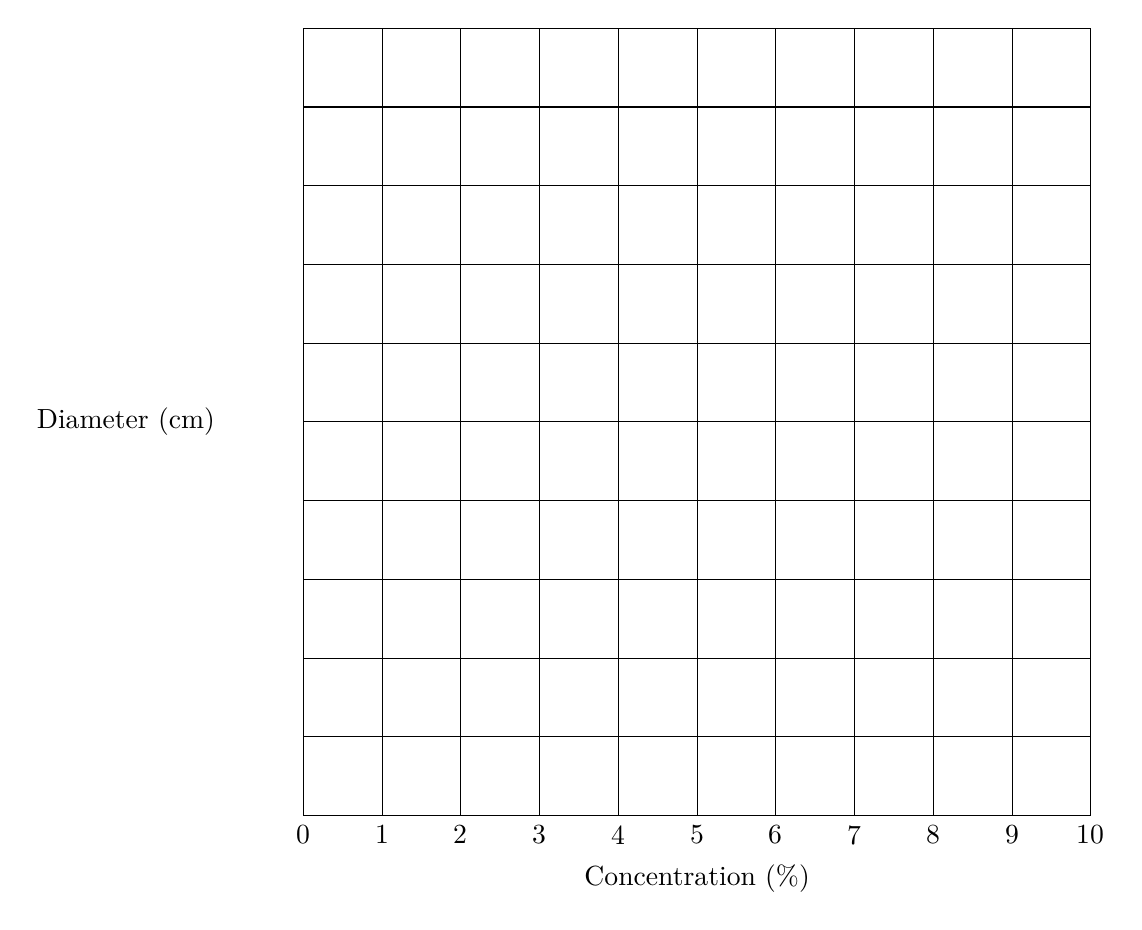
\begin{tikzpicture}
	
		\newcommand*{\xMin}{0}%
		\newcommand*{\xMax}{10}%
		
		\draw (0,0) grid (10,10);
		\draw node [below] at (5,-0.5) {Concentration (\%)};
		\draw node [left] at (-1,5) {Diameter (cm)};
		\foreach \i in {\xMin,...,\xMax}{
			\draw node [below] at (\i,0) {$\i$};
		}

	\end{tikzpicture}

\end{center}

\end{questions}

\subsubsection*{Literature Cited}

\hangpara{\litindent}{1}
Livermore, D.\,M. 2000. Antibiotic resistance to staphylococci. International Journal of Antimicrobial Agents 16 (Suppl. 1): S3–10.

\hangpara{\litindent}{1}
Serafini, A. and D.\,M.\,Matthews. 2009. Microbial resistance to Triclosan: a case study in natural selection. American Biology Teacher 71: 536–540.\footnote{This exercise is based on Serafini and Matthews 2009.}

\end{document}  